\begin{example}
    e.g. An example of a learning problem to understand when the learning algorithm designed is correct or not. \vspace{3.5pt}
    \begin{center}
        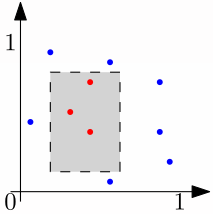
\includegraphics[width = 0.25\textwidth]{img/img10.png}
    \end{center} \vspace{3.5pt}
    Suppose that the data given to the algorithm $A$ are pairs of real numbers, defined as follows:
    $$(x,y) \in R_{[0,1]} \times R_{[0,1]}$$
    where each coordinate has a value between $0$ and $1$. These are labelled as positive or negative depending on being inside or outside a \textbf{rectangle}. \vspace{7pt}

    We would like to learn a classifier that taking in input the whole set of points is able to infer the shape of the grey rectangle. However, the real shape 
    of the final rectangle is unknown, it just knows the color of each point: therefore the learning algorithm should guess, trying several times, providing 
    the rectangle as the output classifier $C$. \vspace{7pt}

    Note: until now we discussed about the computation of the function $f_A$. Remember, only after the computation of the function $f_A$ we will get the classifier
    $C$. \vspace{7pt}

    By the way, the amount of training data could be potentially uncountable and infinite, so there is no hope that the output rectangle it's exactly 
    the one that we are looking for. \vspace{7pt}

    The algorithm $A$ cannot guess the exact rectangle $R$ with perfect accuracy if the data received are too few. As the training data grows in number, we would
    expect the rectangle obtained by $f_A(D)$ converges to $R$, wouldn't we? This is almost impossible, there would be always a little bit of freedom, making 
    the deduced rectangle different from the exact one. \vspace{7pt}

    Instead of defining the correctness of a learning algorithm through this strict equivalance, we can study its behavior as it approaches to the \textbf{limit}.
\end{example}